\documentclass[12pt]{article}
\usepackage[left=2cm, top=2cm, right=2cm, bottom=2cm]{geometry}
\usepackage[utf8]{inputenc}
\usepackage[T1]{fontenc}
\usepackage[french]{babel}
\usepackage{graphicx}
\usepackage{graphics}
\usepackage{amsmath}
\usepackage{tikz}
\usepackage{graphicx}
\usepackage{xcolor}
\usepackage{parskip}
\usepackage{physics}


\title{\textbf{Méthodes expérimentales} \\ TP 2: Collisions}
\author{MENARD Alexandre \\ VIEILLEDENT Florent}

\setlength{\parindent}{1cm}

\begin{document}
\maketitle

\section*{Introduction}
Dans ce travail pratique, on cherche à vérifier la validité de la conservation de la quantité de mouvement 
ainsi que de l'énergie cinétique au cours d'une collision ainsi que mettre en évidence les limites de la conservation énergétique.
Pour cela, on produira des collisions supposées élastiques entre deux chariots avec des conditions initales différentes. On étudiera 
la position et la vitesse de ces derniers pour affirmer ou infirmer
les deux lois. On s'appuiera comme pour les derniers travaux pratiques de Python pour l'analyse et la modélisation de nos données.


\newpage
\section{Étude de différents chocs }

Le but de l'expérience est d'étudier l'énergie cinétique et la quantité de mouvement de deux mobiles avant et après un choc élastique. 

\subsection{Expérimentation}
Pour réaliser les collisions, on utilise un banc de mécanique à niveau, avec deux chariots. On souhaite étudier des collisions élastiques, les chariots sont donc équipés d'aimants, de tel sorte que les chariots ne se touchent pas pendant la choc. Cette configuration permet de limiter l'énergie perdue sous forme de chaleur. Les chariots sont propulsés à la main ou à l'aide d'un propulseur à ressort. 

Concernant la caméra, on la règle sur 30 images par seconde avec ouverture à 1/500s, et permet de capturer la position des deux mobiles au cours du temps.
Enfin, on conservera seulement 4 à 6 images avant et après le choc pour pouvoir négliger les frottements sur ce petit laps de temps. On fixe l'origine de notre repère sur un point entre nos deux mobiles. 

On réalise une première collision élastique en propulsant chaque chariot simultanément avec une vitesse initiale faible.

Pour la seconde collision élastique, un mobile $M1$ est initialement en mouvement et le second mobile $M2$ est immobile.



\subsection{Exploitation des mesures}
Pour nos mesures, l'usage de différents appareils de mesure induit des incertitudes sur nos valeurs. On a:
\begin{itemize}
    \item l'incertitude de la position: $\delta x = 0.005m$ dû au mètre pour la mesure et à l'imprécision du logiciel.
    \item l'incertitude sur le temps: $\delta t = 0.033s$, liée au nombre d'image par seconde. 
    \item l'incertutde sur la masse des chariots: $\delta m_1 =\delta m_2 = 0.0001 kg$, qui est l'incertitude de la balance utilisée. Les valeurs des masses des chariots sont $m1=0.5286\,kg$ et $m2=5282\, kg$.
\end{itemize}

On note respectivement X1 et X2 les positions des mobiles M1 et M2 avant le choc. On note de la même manière X1' et X2' la position des mobiles après le choc. 

\newpage
Après avoir réaliser les expériences, on synthétise les données dans les deux graphiques suivants:
\begin{figure}[h!]
	\begin{center}
		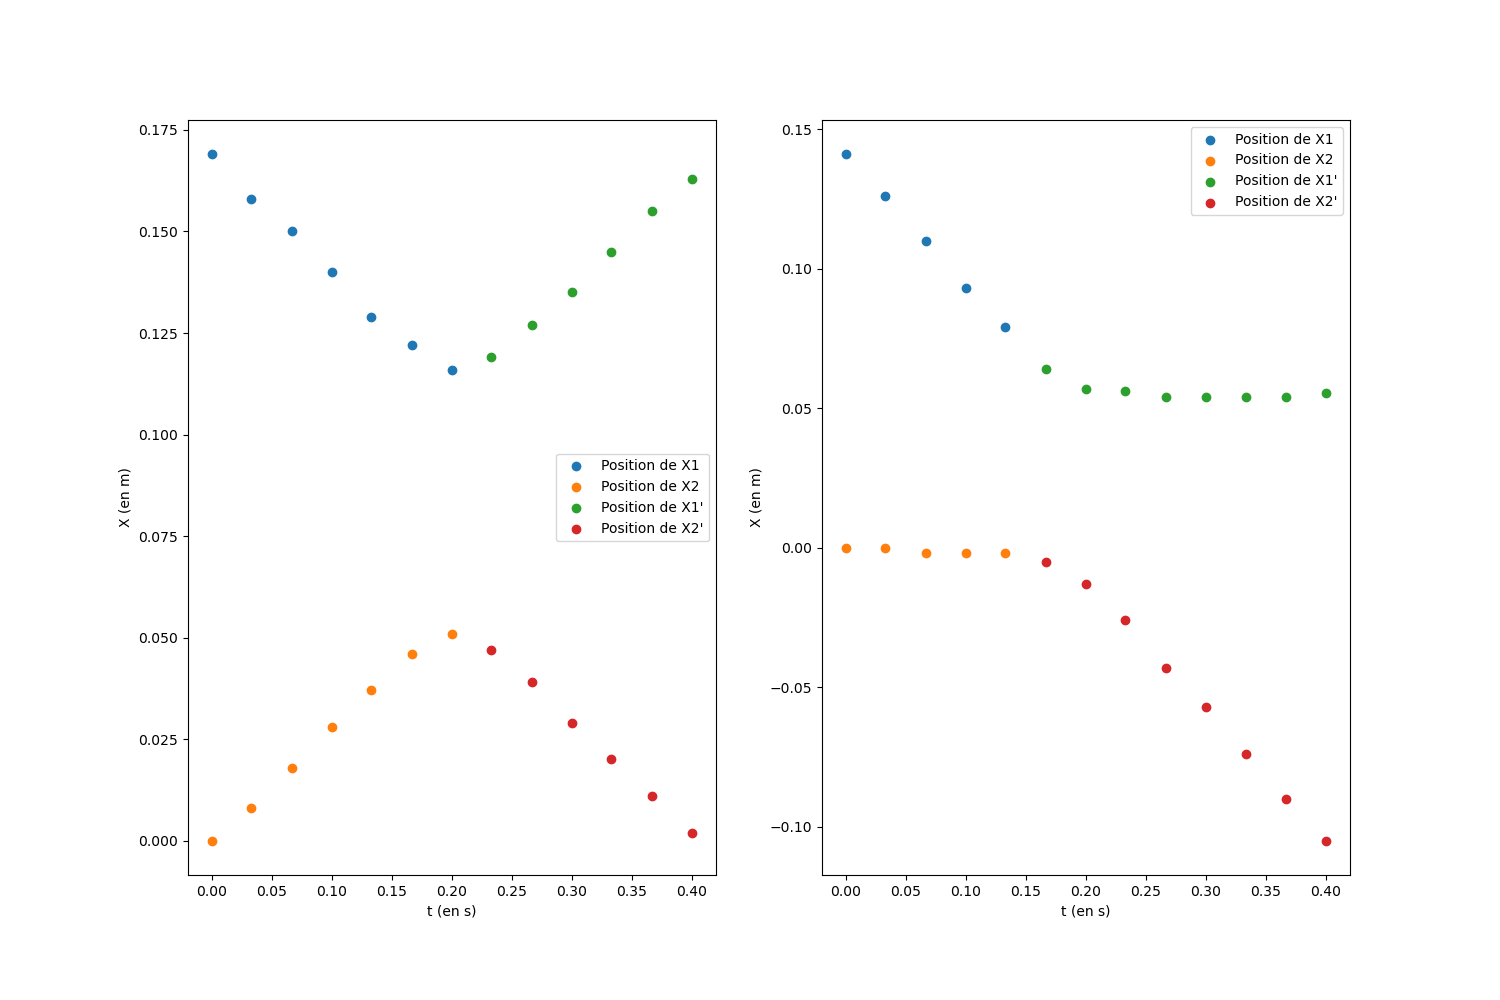
\includegraphics[scale=0.5]{GrapheX.png}
		\label{GrapheX1,...}
		 \caption{Positions des mobiles pour la première expérience(à gauche) et la deuxième expérience(à droite)}
	\end{center}
\end{figure}

On remarque que pour les deux expériences, les points ne se rejoignent pas: c'est parce que le logiciel ne repère pas le bout des mobiles mais un post-it sur le mobile.  

Dans notre expérience, on n'utiliseras pas toutes les valeurs de positions pour calculer les vitesses. On ne cherche pas à calculer les vitesses lors du choc. On calcule donc les vitesses à partir des 4 premières valeurs avant le choc et les 4 dernières valeurs après le choc. 
\newpage
Les valeurs qu'on utiliseras seront donc:
\begin{table}[!h]
	\begin{center}
		\begin{tabular}{|c|c|c|}
		\hline
	
		& Première expérience & Deuxième expérience \\
		\hline
		$X_1^{min}\pm 0.005$ (en m) & 0.169 & 0.141 \\
		$X_1^{max}\pm 0.005$ (en m) & 0.14 & 0.093 \\
		$X_2^{min}\pm 0.005$ (en m) & 0 & 0 \\
		$X_2^{max}\pm 0.005$ (en m) & 0.028 & -0.002 \\
		$X_1^{'min}\pm 0.005$ (en m) & 0.135 & 0.054 \\
		$X_1^{'max}\pm 0.005$ (en m) & 0.163 & 0.056 \\
		$X_2^{'min}\pm 0.005$ (en m) & 0.029 & -0.057\\
		$X_2^{'max}\pm 0.005$ (en m) & 0.002 & -0.105 \\
		$t_{min}\pm 0.033$ (en s) &0 & 0 \\
		$t_{max}\pm 0.033$ (en s) &0.1 & 0.1 \\
		$t'_{min}\pm 0.033$ (en s) &0.3 & 0.3 \\
		$t'_{max}\pm 0.033$ (en s) & 0.4 & 0.4\\
		\hline
		\end{tabular}
		\caption{Données utilisées pour les calculs de vitesses}
		\label{Tabledonnéesutilisées}
	\end{center}
\end{table}

		
Ensuite, on s'intéresse à calculer la vitesse, l'énergie cinétique ainsi que la quantité de mouvement
pour chaque mobile.
Pour calculer la vitesse $v$ à chaque instant $t$, on utilisela formule suivante:
\begin{equation}
    v(t) = \frac{x(t + \delta t) - x(t)}{\delta t}
\end{equation}

On note $t_i, x_i$, l'instant et la position initiale et $t_f, x_f$, l'instant et la position finale. On utilise donc la méthode
des pentes extrêmes pour obtenir l'incertitude sur la vitesse de chaque mobile:
\begin{gather*}
    v_{max} = \frac{(x_f + \delta x) - (x_i - \delta x)}{(t_f - \delta t) - (t_i + \delta t)} \\
    v_{min} = \frac{(x_f - \delta x) - (x_i + \delta x)}{(t_f + \delta t) - (t_i - \delta t)} \\
    \delta v = \frac{v_{max} - v_{min}}{2} \quad v = \frac{v_{max} + v_{min}}{2}
\end{gather*}



On prendra les valeurs absolues de nos résultats pour n'avoir que des vitesses positives.	
		

L'énergie cinétique ainsi que son incertitude sont données par:
\begin{equation}
    E_{ci} = \frac{1}{2}m_iv_i^2 \quad \text{ et } \quad \delta E_{ci} = \frac{1}{2}v_i^2 \times \delta m_i + m_iv_i \times \delta v_i
\end{equation}

Enfin, la quantité de mouvement ainsi que son incertitude sont données par:
\begin{equation}
    p_i = m_iv_i \quad \text{ et } \quad \delta p_i = v_i\delta m_i + m_i\delta v_i
\end{equation}


On regroupe nos calculs dans un tableau:
\begin{table}[!h]
	\begin{center}
		\begin{tabular}{|c|c|c|c|}
		\hline
		Mobile & v(en m/s)  & $E_c$ (en J) & $\rho$ (en $kg.m.s^{-1}$) \\
		\hline
		X2 & $0.6\pm 0.5$ & $0.1\pm 0.2$ & $0.3 \pm 0.3$ \\
		\hline
		X1 & $0.4\pm 0.2$ & $0.04\pm 0.03$ & $0.21\pm 0.08$ \\
		\hline 
		X2' & $0.4\pm 0.1$ & $0.03\pm 0.03$ & $0.19\pm 0.07$\\
		\hline 
		X1' & $0.6\pm 0.5$ & $0.1\pm 0.2$ & $0.3\pm 0.3$\\
		\hline		
		\end{tabular}	
		\label{Tableau première expérience}
		\caption{Valeurs calculées pour la première expérience}
	\end{center}
\end{table}

\begin{table}[!h]
	\begin{center}
		\begin{tabular}{|c|c|c|c|}
		\hline
		Mobile & v(en m/s)  & $E_c$ (en J) & $\rho$ (en $kg.m.s^{-1}$) \\
		\hline
		X1 & $0.7\pm 0.4$ & $0.1 \pm 0.1$ & $0.4 \pm 0.2]$  \\
		\hline
		X2 & $0\pm 0.2$ & $0.002\pm 0.007$  & $0.04\pm 0.08$ \\
		\hline 
		X1' & $0.1\pm 0.2$ & $0.0\pm 0.01$  & $0.06\pm 0.09$ \\
		\hline 
		X2' & $0.7\pm 0.4$ & $0.1\pm 0.1$  & $0.4\pm 0.2$ \\
		\hline		
		\end{tabular}	
		\label{Tableau deuxième expérience}
		\caption{Valeurs calculées pour la deuxième expérience}
	\end{center}
\end{table}

\newpage

Ensuite, on s'intéresse à la conservation de la quantité de mouvement et de l'énergie cinétique du système pour
vérifier les lois de conservation. On note donc $E_c^{tot}$ et $p^{tot}$, l'énergie cinétique et la quantité de mouvement du système. 
Pour les incertitudes, on les somme simplement car les grandeurs d'un mobile sont indépendantes de l'autre mobile. On a par exemple:

\begin{align}
    p^{tot} & = m_1v_1 + m_2v_2 \\
    \Rightarrow \delta p^{tot} & = v_1\delta m_1 + m_1\delta v_1 + v_2\delta m_2 + m_2\delta v_2 \\
    \Rightarrow \delta p^{tot} & = \delta p_1 + \delta p_2
\end{align}

La dérivée de $v_1m_1$ en fonction de $v_2$ ou $m_2$ est nulle. On retrouve exactement le même résultat pour l'énergie cinétique et la vitesse.

\begin{table}[!h]
	\begin{center}
		\begin{tabular}{|c|c|c|c|c|}
		\hline
		& $E_c^{tot}$ (en J) & $E_c^{'tot}$ (en J)& $\rho^{tot}$ (en $kg.m.s^{-1}$) & $\rho^{'tot}$ (en $kg.m.s^{-1}$)\\
		\hline
		Première expérience & $0.1 \pm 0.2$ & $0.1\pm 0.2$ & $0.5\pm 0.3$ & $0.5\pm 0.3$\\
		\hline
		Deuxième expérience & $0.1\pm 0.1$ & $0.1\pm 0.1$ & $0.4\pm 0.2$ & $0.4\pm 0.2$\\
		\hline		
		\end{tabular}
		\label{TableauSomme}
		\caption{Comparaison des sommes d'énergie cinétique et de quantité de mouvement dans les deux expériences}
	\end{center}
\end{table}

\newpage

\subsection{Modélisation}

On fait le bilan des forces pour le choc de deux corps. 
\begin{figure}[!h]
	\begin{center}
		\includegraphics[scale=0.7]{SchémaExp1.png}
		\label{SchmExp1}
		\caption{Schéma de l'expérience}
	\end{center}
\end{figure}


On néglige les forces de frottements. On a donc $\vec{R}=-m\vec{g}$. D'après le PFD, on a :
\begin{align*}
\sum_i\vec{F_i}=m\vec{a}=0\Rightarrow \vec{a}=\vec{0}\Rightarrow v=constante
\end{align*}

Dans un choc élastique, la relation suivante est vérifié:
\begin{equation}
\sum_i E_i=\sum_{j'}E_{j'}
\end{equation}

De même, $m\vec{a}=\frac{d\vec{p}}{dt}$ et $\vec{a}=\vec{0}$, donc:
\begin{equation}
\sum_i \rho_i=\sum_{j'}\rho_{j'}
\end{equation}

On a donc théoriquement que nos sommes d'énergie cinétique et de quantités de mouvement doivent être les mêmes avant et après le choc.
Dans notre cas, on a fait les expériences de telles sortes que les chocs soient élastiques. D'après le tableau (4) nos résultats expérimentaux sont en accord avec la théorie. 

Néanmoins, on a de grandes incertitudes, ce qui réduit l'interprétation possible de nos résultats. On suppose qu'avec des incertitudes plus faibles, les relations d'égalités ne seraient peut-être pas vérifiées, car  on ne peut pas supprimer totalement les forces de frottements et les aimants ne rendent pas  les chocs totalement élastiques.  

\section{Transfert d'énergie cinétique}
Dans cette partie on se propose d'étudier le transfert d'énergie cinétique d'un mobile en mouvement vers 
un mobile au repos. 

\subsection{Théorie}
On suppose donc que le mobile 1 en mouvement de masse $m_1$ avec sa vitesse initiale $v_1$, et le mobile 2 au repos de masse $m_2$ avec sa vitesse initiale
$v_2 = 0 m/s$. On montre que le transfert d'énergie cinétique entre les deux mobiles s'exprime comme:

\begin{equation}
    R = \frac{E^{'}_{c2}}{E_{c1}} = 4 \frac{m_1}{m_2} \left(1 + \frac{m_1}{m_2} \right)^{-2}
\end{equation}

\subsection{Expérimentation}
Pour vérifier le modèle théorique, on lance le mobile 1 avec une vitesse initiale vers le mobile 2 au repos afin de réaliser un choc élastique.
On répéte plusieurs fois la collision en modifiant la masse du mobile 1, et la masse du mobile 2 afin d'obtenir différents rapport de masse $m_1/m_2$ pour comparer avec
le modèle théorique.

On souhaite d'abord reporter la vitesse des mobiles et l'énergie cinétique de ces derniers avant et après la collision. Cependant, on remarque que la vitesse 
fournit par le logiciel n'est pas continu, les valeurs oscillent beaucoup. Pour s'affranchir de ce problème, on décide de prendre la moyenne de la vitesse sur les premières/dernières images
(en prenant soin que la collision ne se produise pas au cours de ces images). Pour les incertitudes, on utilise la méthode des pentes extrêmes entre les deux points qu'on moyenne pour la vitesse et pour les énergies cinétiques, on a:

\begin{gather}
    E_c = \frac{1}{2} m v^2 \\
    \delta E_c = \frac{v^2}{2} \delta m + mv \delta v
\end{gather}

On reporte donc les résultats dans ce tableau:


\begin{table}[h!]
    \begin{center}
        \begin{tabular}{|c|c|c|c|c|c|c|}
            \hline
            R & $v_{i1}$ (m/s) & $v_{f1}$ (m/s) & $v_{f2}$ (m/s) & $E_{ci1}$ (J) & $E_{cf1}$ (J) & $E_{cf2}$ (J) \\ \hline
            0.982 & 0.4 $\pm$ 0.1 & 0.0 $\pm$ 0.4 & 0.33 $\pm$ 0.07 & 0.04 $\pm$ 0.02 & 0.0 $\pm$ 0.005 & 0.03 $\pm$ 0.01 \\ 
            0.914 & 0.4 $\pm$ 0.1 & 0.0 $\pm$ 0.4 & 0.37 $\pm$ 0.07 & 0.04 $\pm$ 0.02 & 0.0 $\pm$ 0.0 & 0.04 $\pm$ 0.01 \\ 
            0.516 & 0.4 $\pm$ 0.1 & 0.1 $\pm$ 0.5 & 0.29 $\pm$ 0.04 & 0.05 $\pm$ 0.03 & 0.0 $\pm$ 0.02 & 0.04 $\pm$ 0.01 \\ 
            0.513 & 0.4 $\pm$ 0.2 & 0.1 $\pm$ 0.5 & 0.3 $\pm$ 0.02 & 0.05 $\pm$ 0.04 & 0.01 $\pm$ 0.04 & 0.045 $\pm$ 0.005 \\ 
            1.020 & 0.6 $\pm$ 0.4 & 0.0 $\pm$ 0.4 & 0.6 $\pm$ 0.3 & 0.1 $\pm$ 0.1 & 0.0 $\pm$ 0.0 & 0.1 $\pm$ 0.1 \\ 
            1.095 & 0.4 $\pm$ 0.2 & 0.0 $\pm$ 0.3 & 0.4 $\pm$ 0.2 & 0.06 $\pm$ 0.04 & 0.0 $\pm$ 0.004 & 0.05 $\pm$ 0.04 \\ 
            1.942 & 0.27 $\pm$ 0.04 & 0.1 $\pm$ 0.3 & 0.33 $\pm$ 0.03 & 0.04 $\pm$ 0.01 & 0.0 $\pm$ 0.02 & 0.028 $\pm$ 0.005 \\ 
            1.951 & 0.4 $\pm$ 0.2 & 0.1 $\pm$ 0.2 & 0.5 $\pm$ 0.3 & 0.1 $\pm$ 0.08 & 0.01 $\pm$ 0.03 & 0.07 $\pm$ 0.08 \\ 
            0.516 & 0.5 $\pm$ 0.3 & 0.2 $\pm$ 0.6 & 0.36 $\pm$ 0.07 & 0.08 $\pm$ 0.08 & 0.01 $\pm$ 0.05 & 0.06 $\pm$ 0.02 \\ 
            0.513 & 0.5 $\pm$ 0.2 & 0.2 $\pm$ 0.5 & 0.27 $\pm$ 0.03 & 0.07 $\pm$ 0.06 & 0.01 $\pm$ 0.04 & 0.038 $\pm$ 0.009 \\ 
            0.914 & 0.4 $\pm$ 0.1 & 0.0 $\pm$ 0.4 & 0.37 $\pm$ 0.08 & 0.05 $\pm$ 0.03 & 0.0 $\pm$ 0.004 & 0.04 $\pm$ 0.02 \\ 
            1.951 & 0.36 $\pm$ 0.05 & 0.1 $\pm$ 0.2 & 0.5 $\pm$ 0.2 & 0.07 $\pm$ 0.02 & 0.01 $\pm$ 0.02 & 0.05 $\pm$ 0.04 \\ 
            \hline
        \end{tabular}
    \end{center}
	\caption{Valeur prise par l'énergie cinétique et la vitesse des deux mobiles avant et après la collision}
\end{table}

\textbf{Remarque:} les énergies cinétiques sont très petites, ce qui explique la présence d'énergies cinétiques à $0$. En réalité, elles ne sont pas toutes nulles,
mais comme la valeur a plus de $0$ après la virgule que l'incertitude, la valeur est arrondie à 0. Cependant, certaines incertitudes valent bien 0 car le mobile 
est bien à l'arrêt, comme c'est le cas dans la deuxième ligne par exemple.

\begin{figure}[h!]
    \begin{center}
        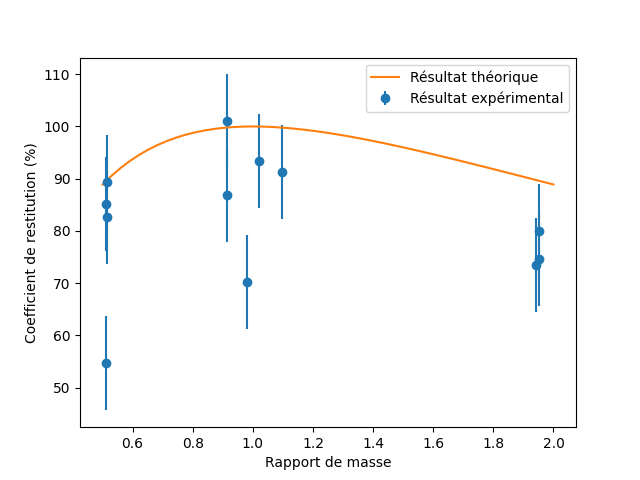
\includegraphics[scale=0.8]{RapportMasse.png}
    \end{center}
    \caption{Comparaison de $R$ entre la valeur théorique et la valeur expérimentale}
\end{figure}

Pour déterminer l'incertitude sur $R$ due à la force entre les aimants qu'on ne peut mesurer, nous avons répété plusieurs fois la même situation à un même rapport de masse, 
et on a obtenu un écart de $R$ d'environ 10\% que l'on a reporté sur le graphique ci-dessus.

\newpage
On remarque sur le graphique un écart considérable entre la valeur théorique et la valeur expérimentale. Cet écart peut s'expliquer par notre hypothèse, où l'on suppose le choc parfaitement élastique, alors
que les chocs ne sont jamais totalement élastique, ce qui invalide notre hypothèse initiale. De plus, pour approcher des conditions d'un choc élastique, les chariots ne collisionnent pas réellement, mais le choc se produit
au travers d'aimant qui se repousse entre eux. La force entre les deux aimants est indépendante et l'on ne peut pas la mesurer, on ne peut donc pas estimer l'incertitude dessus, et quantifier si cette force 
peut totalement "transmettre" l'énergie du mobile 1 au mobile 2. Il y a donc un flou conséquent sur cette partie du choc que l'on ne peut déterminer.

Finalement, en regardant le graphique, on peut se demander quelles sont les conditions pour maximiser le transfert, ou à l'inverse, le minimiser. On remarque sur la courbe que le transfert est maximal lorsque
le rapport de masse est proche de 1, donc lors d'un choc entre deux masses équivalentes, et minimal lorsque le rapport de masse s'éloigne de 1, donc lors d'un choc entre une masse très grande devant l'autre.

\section{Conclusion}

\end{document}
